\chapter{Designing and Implementing the OurPlace Platform}
\label{chap:Design}

Following the engagements covered in Chapter \ref{chap:DesignSpace}, I decided to iterate upon the Park:Learn prototype application. With the aim of creating an application which could be utilised in formal and informal learning contexts, I examined previous mobile learning research (summarised in Chapter \ref{chap:MobileLearning}) to produce a number of design goals for the technology. This application would also aim to follow the implications for design (as described in section \ref{sec:SuggestionsCivicLearning}) derived from the findings of the previous exploratory study. This chapter describes the design goals for the technology, why those goals were chosen, a detailed overview of the application itself and how it evolved over the course of the remainder of the project. 

Much of the work covered by this chapter was peer-reviewed and published at MobileHCI 2018 \citep{Richardson2018}, with the paper being co-authored by Doctors Pradthana Jarusriboonchai, Kyle Montague and Ahmed Kharrufa. 

\section{Technology Design Goals}
\label{sec:DesignGoals}
Based on the findings of previous works and the design engagements covered in Chapter \ref{chap:DesignSpace}, we produced several design goals (DGs). This section describes each design goal and the rationale behind choosing them.

% reference like this: (addresses \hyperref[DG1]{DG1})

\subsection*{ DG1: Utilize local places and communities as learning resources }
\phantomsection
\label{DG1}

This first goal is that the final technology should support greater utilisation of local places (e.g. parks, buildings, towns, rooms, etc) and the communities which surround, inhabit and have built relationships with them as learning resources. This primarily relates to the previously discussed Park:Learn studies, during which we found that places' stakeholders can offer not only a diverse knowledge base, but also a large variety of motivations, aspirations and tensions related to place. We suggested that mobile learning technologies might be able to make use of these social infrastructures, by giving places’ stakeholders a platform for sharing their values through designing and sharing learning activities in authentic contexts \citep{Richardson2017}. This would not only support learners in situating their learning activities within authentic physical environments, but might also introduce them to new communities of practice which they may enter and develop an expertise through interactions with them \citep{lave1991situated}.

\subsection*{ DG2: Support seamless outdoor and classroom use }
\phantomsection
\label{DG2}

As noted by Sharples, mobile learning does not necessarily always take place in one context, or even one fixed level of formality \citep{Sharples2013}. He presents mobile learning as taking place on a linear spectrum: from formal, classroom and curriculum-based learning activities, to ones are informal, creative and \textit{mobile} [Figure \ref{fig:learningContextDimension}]. However, while these contexts are different, they can still be connected---Kuh argues that learning experiences across contexts can be bound into a `seamless learning' narrative \citep{Kuh1996}. In order to support this seamless use across contexts, our design should encompass as many of Wong and Looi's `desirable dimensions' of seamless learning as possible \citep{Wong2011} (all ten dimensions are listed in section \ref{sec:Seamless}). Multiple examples of seamless mobile learning applications which adhere to some (or all) of these dimensions already exist. For example, Zydeco supports the use of multiple types of devices across multiple locations (classrooms and museums), utilising both digital and physical learning resources \citep{kuhn2011}.

\subsection*{ DG3: Support a variety of pedagogical approaches and stakeholder requirements }
\phantomsection
\label{DG3}

The final `desirable dimension' listed by Wong and Looi is that seamless mobile learning technologies should encompass multiple pedagogical models, as a diversity of learning experiences requires the deployment of different learning models \citep{Wong2011}. For example, the learning theory of constructionism and project-based learning pedagogies (as covered in section \ref{sec:ConstructionismPBL}) have different requirements to more traditional classroom teaching methods. Sessions within these pedagogies will often have different goals, with the intended outcomes also changing according to the stakeholders' agenda (e.g. as discussed Chapter \ref{chap:DesignSpace}, teachers may want to be able to provide evidence of students' learning, while park rangers and volunteers may want to promote place-making in an attempt to nurture stewardship and volunteerism). As such, our technology needs to be flexible enough to support different goals, learning processes and intended outcomes, ideally without relying heavily on additional tools.

\subsection*{ DG4: Support a wide range of user ages and technical expertise }
\phantomsection
\label{DG4}

While it has almost become a truism that children are frequently technologically adept, care still needs to be taken to support age and ability groups who may struggle with reading or typing large quantities of text (as shown to be an issue in MyArtSpace \citep{Vavoula2009} and deliberately avoided in Zydeco \citep{kuhn2011}). Furthermore, engaging with a large variety of place stakeholders means that older age groups---who may not be as technologically literate---may wish to use the technology. Our technology design should therefore strive to minimise (or provide alternatives to) large amounts of typing, and, as suggested by Land, attempt to support a range of learner ages and reading abilities through the use of simple, varied but semantically consistent visual interfaces \citep{Land2015}.

\subsection*{ DG5: Support learning and reflection in authentic learning contexts }
\phantomsection
\label{DG5}

Our observations in the initial engagements (as well elements found in prior work, such as in Mobilogue \citep{Giemza2013}) demonstrated that giving students greater control and opportunities for creativity can act as a motivating factor. As such, our design aimed to utilise interaction methods on mobile devices which support student creativity and control in authentic learning environments. That said, while not all mobile learning projects make use of the learner's context as a learning environment or resource \citep{Frohberg2009}, even fewer promote learner reflection within the authentic learning environment. For example, MyArtSpace \citep{Vavoula2009} and Sense-It \citep{Sharples2017} encourage learners to use the technology to collect data or take brief notes and observations, rather than engage in in-depth reflection in-situ. This is certainly useful, and should have a place in the final design. However, we wanted our design to also support immediate reflection from the learner, without the need to return to the classroom. This level of immediacy should also apply to activity creation and data collection, in an attempt to minimise the learner being distracted from authentic engagement with the learning context. 

\subsection*{ DG6: Support mobile learning in resource-limited schools }
\phantomsection
\label{DG6}

As discussed in sections \ref{sec:DigitalCivics} and \ref{sec:ParkContext}, the UK as a whole is enduring an extended period of austerity and local authorities have had to cut funding wherever possible. As a result, many schools have become resource-limited and may struggle to justify spending money on having more smart mobile devices for classroom use, despite them becoming more affordable and fashionable within education. While our final software design will require the use of a smartphone or tablet, it must take steps to minimise the financial strain placed upon schools in its use. The design should: require minimal teacher time to set up and use, as well as access and download student work; support the sharing of devices between multiple students, either through group work or the ability to save and clear progress to allow another student to start activities afresh (as seen in Mobilogue \citep{Giemza2013}); and support the offline caching of data, allowing teachers to pre-load content in the classroom prior to trips, or queuing student work for later upload (avoiding expensive 4G mobile data contracts).

\section{An Overview of ParkLearn and OurPlace}

ParkLearn, the prototype application discussed in Chapter \ref{chap:DesignSpace}, was further developed to meet these design goals. While the early version was created as a simple proof of concept and acted as a technology probe, later versions featured far greater functionality. This section will detail the application: its features, its implementation, and how it evolved over time into the later OurPlace app. As the two versions are extremely similar, for the sake of clarity `OurPlace' will be used as the application's name for the rest of this chapter. Significant differences in the two applications' features or implementations will be noted explicitly.

The main screen of the OurPlace app consists of two main sections, separated by tabs: `Highlights', which shows public content created by all users, and `My Creations', which lists the Creations (Activities and/or Collections, defined below) created by the current user. This section details the nature of this content, how it is experienced by learners, how users can create their own, and how it can be shared with others.

\subsection{The Anatomy of an Activity}
\label{sec:ActivityOverview}
Core to the OurPlace application is the concept of `Activities'. In terms of user interaction, they are very similar to the ones introduced in the prototype ParkLearn application, which were based on the original jigsaw workshop activity [Figure \ref{fig:rangerJigsaw}]. While the Activities in the prototype version were hard-coded into the application, later versions allowed users to create their own Activities, or complete other people's. They are delivered to the mobile app by the remote server in the standard JSON data format (see section \ref{sec:ImplementationWeb}), allowing for the app to allow users to discover and open Activities in numerous ways (see section \ref{sec:SharingActivities}).

\begin{figure*}
  \centering
  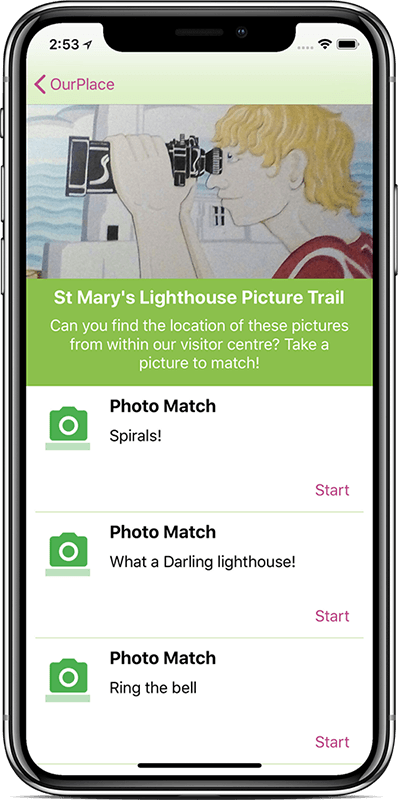
\includegraphics[width=0.45\columnwidth]{images/chapter05/activity.png}
  \caption[A simple OurPlace Activity]{ A simple Activity in the OurPlace iPhone app. The Activity's image, title and description appear at the top, with Tasks underneath. The Task Type of each Task is made known to the user by displaying its name and icon (i.e. `\textit{Photo Match}'). The screen can scroll vertically if there are more Tasks than can be displayed at once.}~\label{fig:ActivityExample}
\end{figure*}

Activities are typically based on a particular topic, location or subject (e.g. `\textit{Exploring the Rose Garden}'). Each OurPlace Activity must feature a title and a short (up to 150 characters) description, which gives the learner some insight into what the Activity will be about [Figure \ref{fig:ActivityExample}]. Additionally, Activity creators may choose to include an image to represent the Activity: this will appear on the application's feeds, and at the top of the main Activity screen. The application supports taking this image directly through the device's camera, or the use of pre-existing images from the user's photo gallery (allowing users to select images they prepared earlier, or downloaded from the Internet). By allowing both options, activity creators are able to either create their Activities within the relevant physical context (addresses \hyperref[DG5]{DG5}) or remotely, which may be easier if preparing for a future school trip (addresses \hyperref[DG6]{DG6}).

Each Activity must also feature at least one `Task'. Tasks are small, modular pieces of content centring around one of a number of pre-defined user interactions (e.g. `\textit{Take a Photo}'). A large number of variations (`Task Types') of Tasks are available, supporting a berth of different interactions (addresses \hyperref[DG3]{DG3}). Section \ref{sec:TaskTypes} describes all of the different Task Types available in OurPlace (note that `\textit{Scan the QR Code}' was introduced in OurPlace, and was not available in ParkLearn). An Activity can have an unlimited number of Tasks, and the learner is able to complete them in any order.

As noted in Chapter \ref{chap:DesignSpace}, each of these interactions were chosen either because they put an element of creative control into the hands of the learner (\textit{Take a Photo, Draw a Picture, Draw on Photo, Record Video, Record Audio}) (addresses \hyperref[DG5]{DG5}), took advantage of the devices’ hardware capabilities across different contexts (\textit{Listen to Audio, Map Marking, Location Hunt, Scan the QR Code}) (addresses \hyperref[DG2]{DG2}), emulated features of the learning materials already in use by teachers and park rangers (\textit{Information, Multiple Choice, Text Entry}) (addresses \hyperref[DG3]{DG3}), or a combination of all of the above.

\begin{figure*}
  \centering
  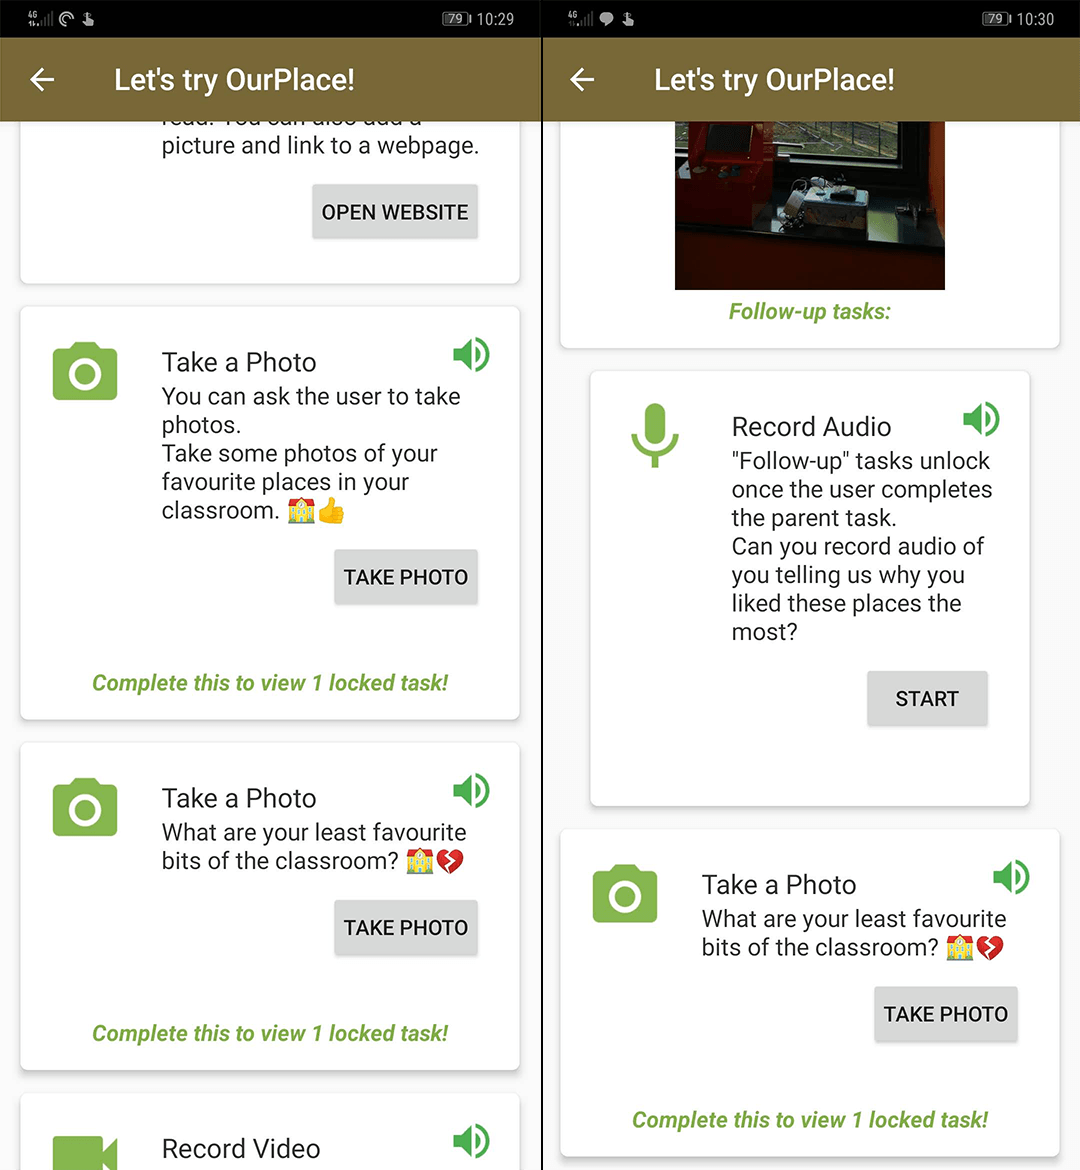
\includegraphics[width=0.6\columnwidth]{images/chapter05/FollowUpTasks.png}
  \caption[Follow-Up Task example]{An example of how Follow-Up Tasks work. Completing `parent' Tasks (left) makes any Follow-Up Tasks they might have available to the learner. Follow-Up Tasks are listed below the parent, and appear on slightly smaller cards to make them visually distinct (right). }~\label{fig:FollowUpTasks}
\end{figure*}

The OurPlace app also features the concept of `Follow-Up Tasks', which were not available in ParkLearn. Follow-Up Tasks act as children to a chosen parent Task, only becoming available when the parent has been marked as completed by the system [Figure \ref{fig:FollowUpTasks}]. For example, a Task might ask the learner to take a picture of the item in a museum they found most interesting, and then a Follow-Up Task could ask them to record an audio clip of them explaining what was interesting about it. We hope that having this ability allows Activity designers to encourage students to reflect through the application, whilst still being situated in the authentic learning environment (addresses \hyperref[DG5]{DG5}). In order to make learners aware of locked Follow-Up Tasks, a `\textit{Complete this to view X locked tasks!}' message is displayed upon the parent Task [Figure \ref{fig:FollowUpTasks}, left]. Once the parent Task has been completed, the message changes to `\textit{Follow-Up Tasks:}' and the child Tasks are listed below the parent [Figure \ref{fig:FollowUpTasks}, right]. To make the Follow-Up Tasks visually distinct, they appear on slightly smaller cards in the app's interface than their parents. Once completed, Tasks cannot be `uncompleted' (e.g. by deleting all taken photos), meaning that unlocked Follow-Up Tasks will remain available unless the Activity's progress is completely reset.


\subsection{Overview of Task Types}
\label{sec:TaskTypes}
Below are all of the Task Types available to users creating Activities in the OurPlace application. Unless noted otherwise, the functionality of each Task Type was identical between ParkLearn and OurPlace. All Task Types contain a some sort of textual description or instruction, with a `text to speech' button which reads the description aloud when pressed. If a Task has an interaction for the learner to perform, it will either be assigned to an `action button' (e.g. `TAKE PHOTO' and `START' in Figure \ref{fig:FollowUpTasks}) which will navigate to a new screen in the app, or take place on the Activity's main screen (e.g. Multiple Choice and Text Entry in Figure \ref{fig:TaskTypes3}). 

\begin{figure*}
  \centering
  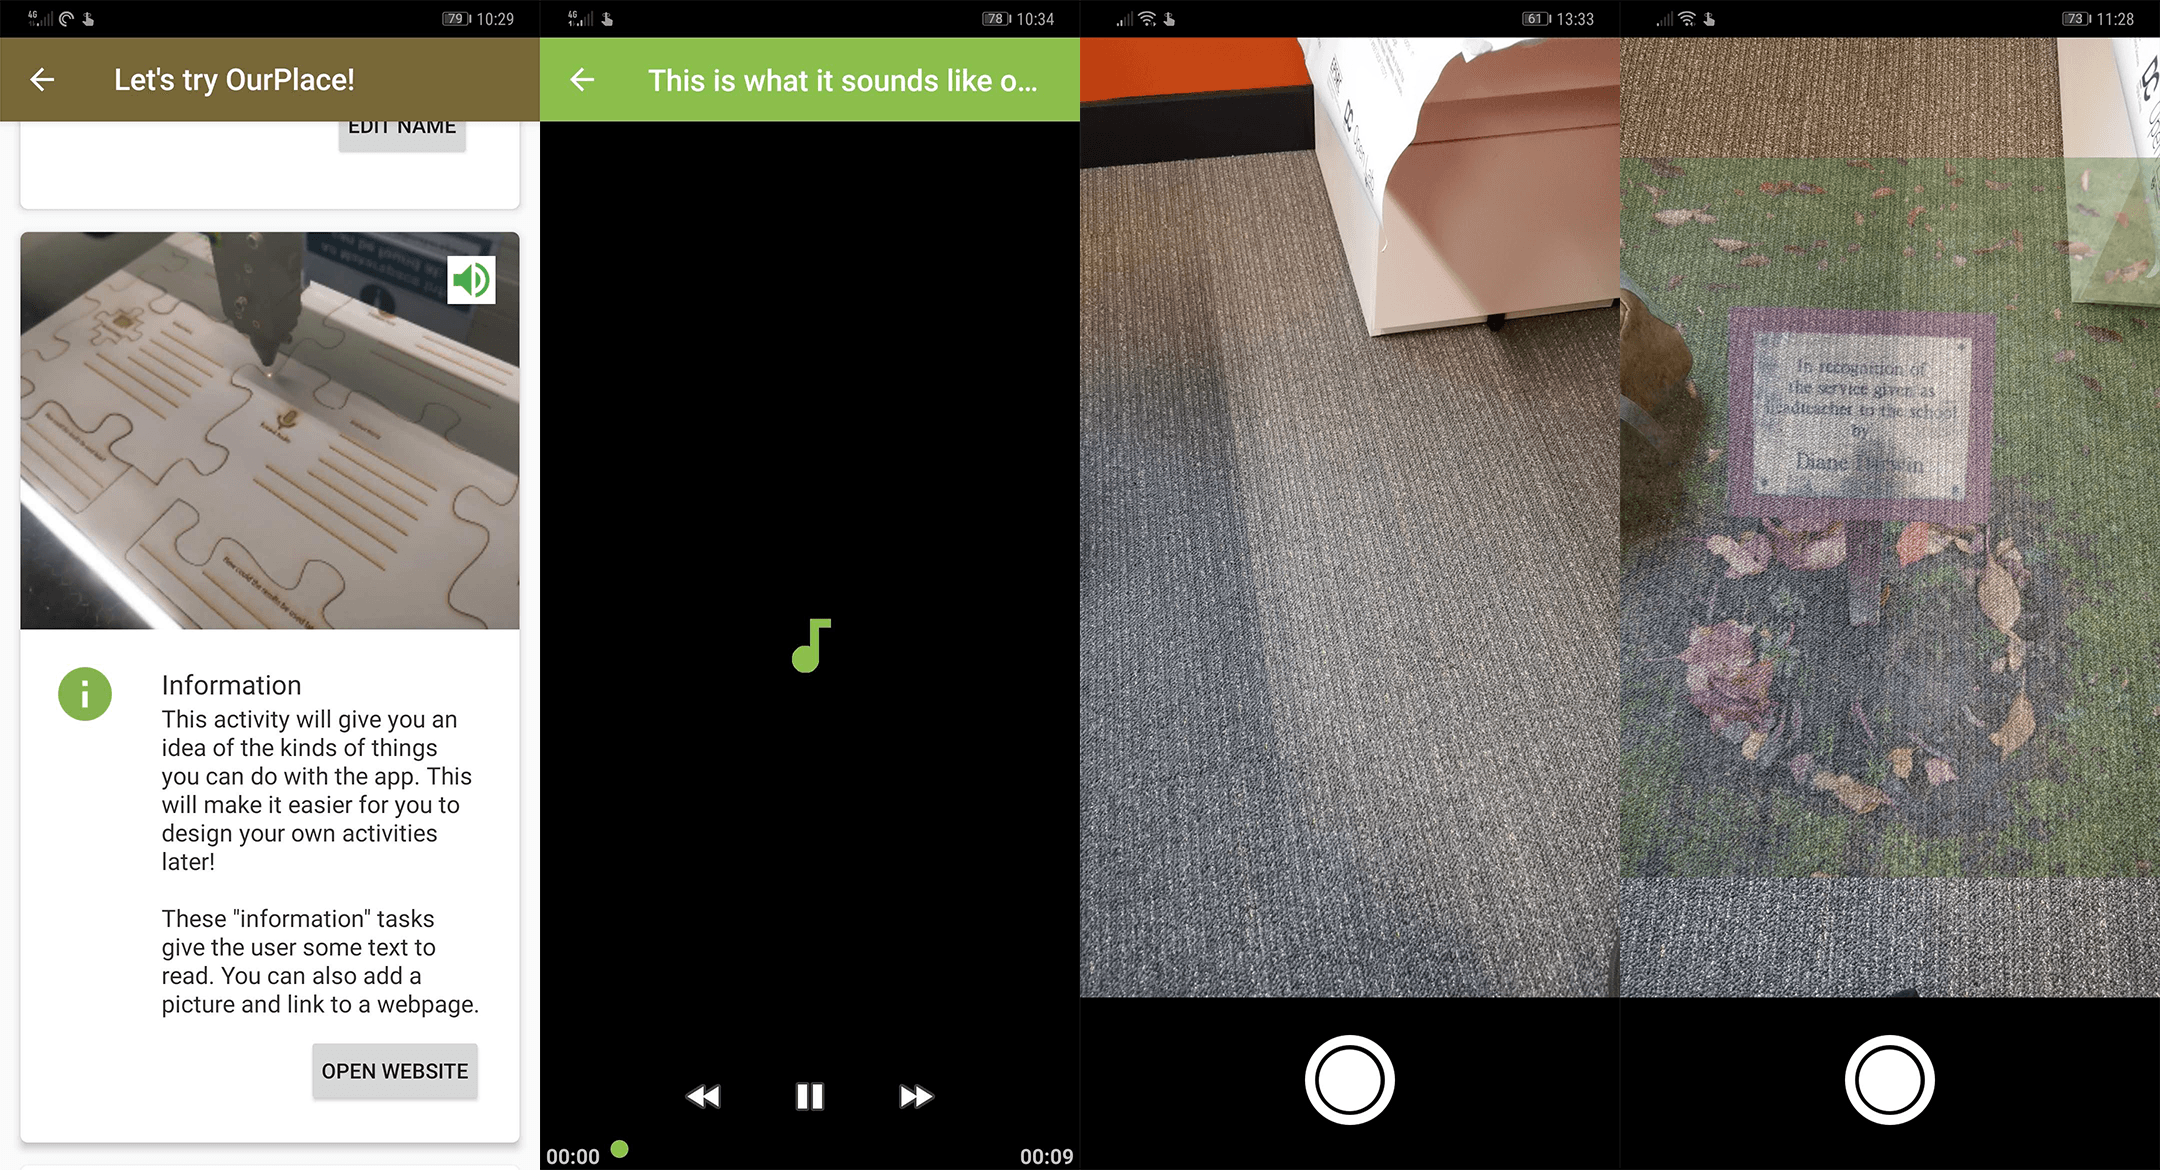
\includegraphics[width=1\columnwidth]{images/chapter05/tasktypes1.png}
  \caption[Task Types (part 1)]{Task Types (left to right): a) Information; b) Listen to Audio; c) Take a Photo; d) Photo Match}~\label{fig:TaskTypes1}
\end{figure*}

\subsubsection*{Information}
One of the simplest Task Types, this presents the learner with a piece of text to read. Optionally, the Activity author can also choose to include an image to accompany the text, as well as a hyperlink to a related web page. If included, the hyperlink is assigned to the Task's action button, which will open the address in the device's default web browser when pressed [Figure \ref{fig:TaskTypes1}.a]. because they are passive (and the action button is optional), Information Tasks are marked as completed by default, meaning any Follow-Up Tasks are immediately visible.

\subsubsection*{Listen to Audio}
The learner is given an audio recording to listen to. Tapping the Task's action button will open up a media player screen, where the audio file plays on a loop until closed [Figure \ref{fig:TaskTypes1}.b]. The Task is marked as completed when the media player is closed. The original ParkLearn application was slightly different, in that the audio played from the Activity's main screen, with a simple `stop' button being shown on a pop-up. The OurPlace implementation improves upon this by allowing the user to `scrub' through the audio file to any given timestamp.
    
\subsubsection*{Take a Photo}
This Task Type asks the learner to take one or more photos of a subject. The action button opens up a simple camera screen [Figure \ref{fig:TaskTypes1}.c]. Whilst mobile applications would normally use the device's default camera application, the app's other camera-related Task Types have more complex requirements, requiring custom solutions. For the sake of consistency, that custom camera screen is also used for this simpler interaction (\hyperref[DG4]{DG4}). When a photo is taken, the camera closes and returns to the Activity screen. Multiple photos can be taken, and are listed below the Task's action button [Figure \ref{fig:MediaViewer}.a]. Tapping one of these will open it in the media viewer screen, where the user can see a larger view of the photo, with the option to delete it by tapping a bin icon [Figure \ref{fig:MediaViewer}.b]. The original ParkLearn app did not have this media viewer screen, however unwanted photos could still be deleted through a `tap and hold' interaction on the images.

\begin{figure*}
  \centering
  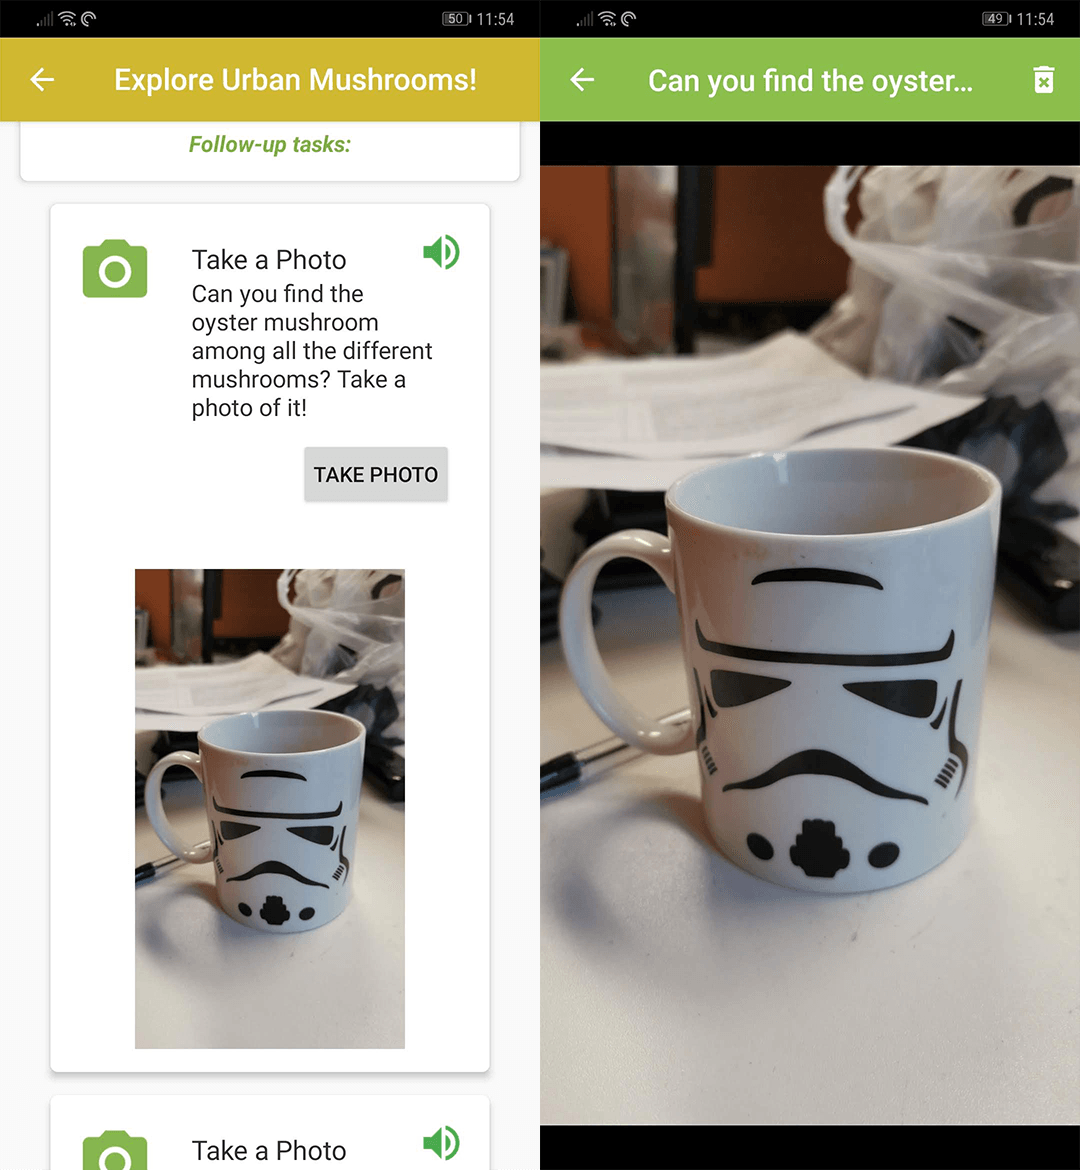
\includegraphics[width=0.55\columnwidth]{images/chapter05/mediaViewer.png}
  \caption[OurPlace's media viewer]{(left to right): a) Resulting images from `Take a Photo' are listed below the Task on the Activity screen. b) Tapping one opens it on the media viewer screen, where the option to delete the item is available.}~\label{fig:MediaViewer}
\end{figure*}

\subsubsection*{Photo Match}
This is similar to `Take a Photo', in that the learner is asked to take one or more photos of a subject. However, the camera screen shows a semi-transparent overlay of another image on top of the camera feed [Figure \ref{fig:TaskTypes1}.d]. The Activity author provides an image of their own choosing (e.g. a photo they have taken, or downloaded from the Internet). Viewing and deleting resulting images is handled the same as in Take a Photo. This extremely basic form of augmented reality is simple enough for users to configure themselves, while still hopefully supporting the grounding of the digital content in the physical environment \citep{javornik2019}. 

\begin{figure*}
  \centering
  \includegraphics[width=1\columnwidth]{images/chapter05/tasktypes2.png}
  \caption[Task Types (part 2)]{Task Types (left to right): a) Draw a Picture; b) Draw on Photo; c) Record Video (rotated); d) Record Audio}~\label{fig:TaskTypes2}
\end{figure*}

\subsubsection*{Draw a Picture}
The learner is asked to draw a picture, using a basic painting interface which is launched by tapping the Task's action button. A wide variety of colours can be selected using the selector at the top of the screen, and drawn onto a blank white canvas [Figure \ref{fig:TaskTypes2}.a]. Tapping the save icon will save the drawing as a JPEG file and return to the Activity screen, where it can be viewed/deleted in the same way as photo files. Multiple drawings can be made.

\subsubsection*{Draw on Photo}
Functionally the same as `Draw a Picture', however the blank white canvas is replaced by a supplied image [Figure \ref{fig:TaskTypes2}.b]. The Activity author can either provide an image of their own choosing (e.g. a photo they have taken, or downloaded from the Internet), or---if this is a Follow-Up Task to an appropriate parent, such as a Take a Photo or Photo Match---have the overlay be one of the images taken by the learner in the parent Task. Images can be viewed and deleted in the same way as other photos and drawings.

\subsubsection*{Record Video}
Learners are asked to record a video of a subject using the camera, which is launched by tapping the action button. The camera screen is locked in the landscape orientation, and features a help button which will show the Task's description/instruction when pressed [Figure \ref{fig:TaskTypes2}.c]. Recording starts when the shutter button is tapped, at which point the button turns red. To minimise storage issues, a custom video recorder screen was implemented, which caps video recordings at 10 minutes in length and at a 720p resolution (\hyperref[DG6]{DG6}). When the shutter button is pressed again (or the 10 minutes elapses), the video is saved and the user is returned to the Activity screen. Multiple videos can be recorded, and thumbnails for each are listed below the Task (as with the photo results). Tapping a video file will open it in the media screen, where it can be replayed and deleted as desired.

\subsubsection*{Record Audio}
Learners are asked to record an audio clip using the device's microphone. Tapping the action button opens a separate recording screen, showing a start/stop record button, record timer and the current Task's instruction for easy reference [Figure \ref{fig:TaskTypes2}.d]. After pressing stop to finish the recording, the learner can immediately listen back to it and confirm they're happy with it. If content, learners can save the file, which returns them back to the Activity screen. Recorded audio clips are listed below the task: tapping one will open it in the media screen, where it can be replayed and deleted as desired.

\begin{figure*}
  \centering
  \includegraphics[width=1\columnwidth]{images/chapter05/tasktypes3.png}
  \caption[Task Types (part 3)]{Task Types (left to right): a) Map Marking; b) Location Hunt; c) Multiple Choice; d) Text Entry}~\label{fig:TaskTypes3}
\end{figure*}

\subsubsection*{Map Marking}
This is the only Task Type which requires an active Internet connection during use, and so was the least frequently used in every study. It asks learners to mark a given number of locations onto a Google Map [Figure \ref{fig:TaskTypes3}.a]. The user's current location is shown on the map by a blue dot. Map markers can either be placed on the user's current location, or at custom locations by the learner tapping the map. If they desire, the Activity's author can restrict the learner to only placing markers on their current location, meaning that learners have to physically travel to places they want to mark. Learners can deleted markers they've placed by tapping them. The Activity author can also configure the minimum and maximum number of markers the learner is required to put down before completing the Task (can be set as unlimited by putting a zero as the maximum). Completing the Task will result in a small, non-interactive version of the map being shown under the Task on the Activity screen. When tapped, this will re-open the full map for editing. There were plans to re-engineer this Task Type to use OpenStreetMap instead of Google Maps due to its support for offline caching, however this didn't come to fruition due to time limitations.

\subsubsection*{Location Hunt}
This uses the device's GPS, like Map Marking, but doesn't require an active Internet connection as it doesn't display a map. Instead, learners are asked to track down a target location by observing their device's distance from the target coordinates [Figure \ref{fig:TaskTypes3}.b]. A large graphic performs a `breathing' animation, getting faster/slower as the user gets closer/further away from the target. A beep is also played each time the animation loops, giving the impression of a `GPS metal detector'. The device's current GPS accuracy (in metres) is also given for context, so that the learner can be aware of poor signal (e.g. if they're indoors). Once the learner is within 10 metres of the target, a pop-up notification is shown notifying them of their arrival, and the Task is marked as completed. The OurPlace app introduced the ability for Activity authors to choose to allow learners to open up a route to the target location in Google Maps should they wish, however doing so requires an active Internet connection.

\subsubsection*{Scan the QR Code}
Learners are asked to find and scan a specific QR (Quick Response) code, with the Task's instruction ideally acting as a clue to find it. Tapping the action button opens up the application's built-in QR code scanner. Scanning the wrong code shows a failure message (`\textit{That's not it!}'), while finding and scanning the correct code completes the Task. The Activity's author can view and print the generated QR codes from the OurPlace website. This Task Type was introduced in OurPlace, primarily to support `Location Hunt' style Tasks indoors, where GPS might not work properly.

\subsubsection*{Multiple Choice}
Learners are asked to choose one of (at least two) different text options. Options are presented as a list of radio buttons on the main Activity screen [Figure \ref{fig:TaskTypes3}.c]. The Task is marked as completed once an item is chosen.

\subsubsection*{Text Entry}
Learners are asked to enter some text into a text field on the main Activity screen [Figure \ref{fig:TaskTypes3}.d] using the device's default virtual keyboard. Virtual keyboard apps vary per device, with some also allowing for `voice typing', where learners can speak into the microphone for real-time text transcription. Regardless of input method, the Task is marked as completed once at least one character has been entered into the text field. 

\subsection{Completing Activities}

Once Activities are opened, they (and the files they depend on, such as images and audio) are cached by the application so that they can be accessed without an Internet connection. By default the app caches up to four Activities at a time, cycling them out according to date last accessed. This default limit was put in place to avoid taking up too much device storage with old Activities, however it can be increased up to 20 cached Activities in the app's settings. These features were implemented to address \hyperref[DG6]{DG6}.

Tasks within Activities (with the exception of Follow-Up Tasks, until they are unlocked) can be completed in any order. The learner can tap `Finish' to complete the Activity at any time, even if there are Tasks which have not been completed. ParkLearn initially required that all Tasks be responded to, however this resulted in teachers and researchers entering `junk' data in order to upload responses by students who hadn't responded to each Task during a session. After the learner taps Finish, the application checks if there are responses to upload (e.g. entered text, photos, audio clips etc). If there are, these are packaged up and added to an upload queue, and the user's progress through the Activity is reset to allow another learner to start it afresh. This allows for multiple students to use the same device, without having to overwrite each others' work (\hyperref[DG6]{DG6}). Having an upload queue also allows for teachers to upload the student's work on return to the classroom, avoiding the need for slow and costly mobile data plans (also addressing \hyperref[DG6]{DG6}). Once the learners' data has been uploaded, the local version of it is deleted to free up storage space.

If the Activity was made by another user, once Finish is tapped the application will also ask the learner if they wish to share their results/creations with the Activity's author. If they agree, the Activity's author will be able to see the uploaded data on the OurPlace website (discussed in Section \ref{sec:ImplementationWeb}). Otherwise, only the learner will be able to see the uploaded data. Making Activity responses private uploads by default was a conscious decision, made to support schools' use of learning materials generated by external communities, while simultaneously preventing the accidental sharing of images of children outside of the school (\hyperref[DG2]{DG2}). 

\subsection{Creating Activities}

To make Activity creation as accessible and intuitive as possible, the entire process takes place inside of the OurPlace mobile app. This means no additional equipment is required, and allows the designer to create the Activity in situ if they wish (addresses \hyperref[DG1]{DG1}, \hyperref[DG2]{DG2}, \hyperref[DG5]{DG5}). That said, should the author require their Activity to contain media of a higher degree of quality than can be produced through their mobile device's hardware, the app also supports importing media from external sources (e.g. Google Drive, Dropbox). This means that if the author has access to high quality production hardware and software (e.g. DSLR cameras, studio microphones), they can produce their Activity's media separate from the device and import it into the OurPlace app. This means that while Activity creation has a low barrier to entry, those who have the means and inclination to go the extra mile and produce more `professional' Activities are able to do so (\hyperref[DG3]{DG3}, \hyperref[DG4]{DG4}). This also has the added benefit of users being able to use media that they've downloaded from the Internet (e.g. Google Images). While on a large-scale commercial platform this would likely raise issues around misuse of intellectual property, we decided to overlook the issue due to the small nature of our deployments and lack of monetisation.

To make the experience of creating Activities as consistent as possible, the process uses the same iconography and similar functionality and layouts to the ones seen by learners when completing Activities. For example, as in the Activity `consumption' view, the Activity's details are shown at the top of the screen, with its Tasks laid out in a list below [Figure \ref{fig:ActivityCreation}]. This means that introducing users to the application through consuming an example Activity will partially prepare them for the creation process (addresses \hyperref[DG4]{DG4}). After supplying a title, description and an optional image [Figure \ref{fig:ActivityCreation}.a], the designer creates the Tasks that make up the Activity. Each Activity requires at least one Task before it can be uploaded. Tasks can be re-ordered by dragging them up or down the list.

\begin{figure*}
  \centering
  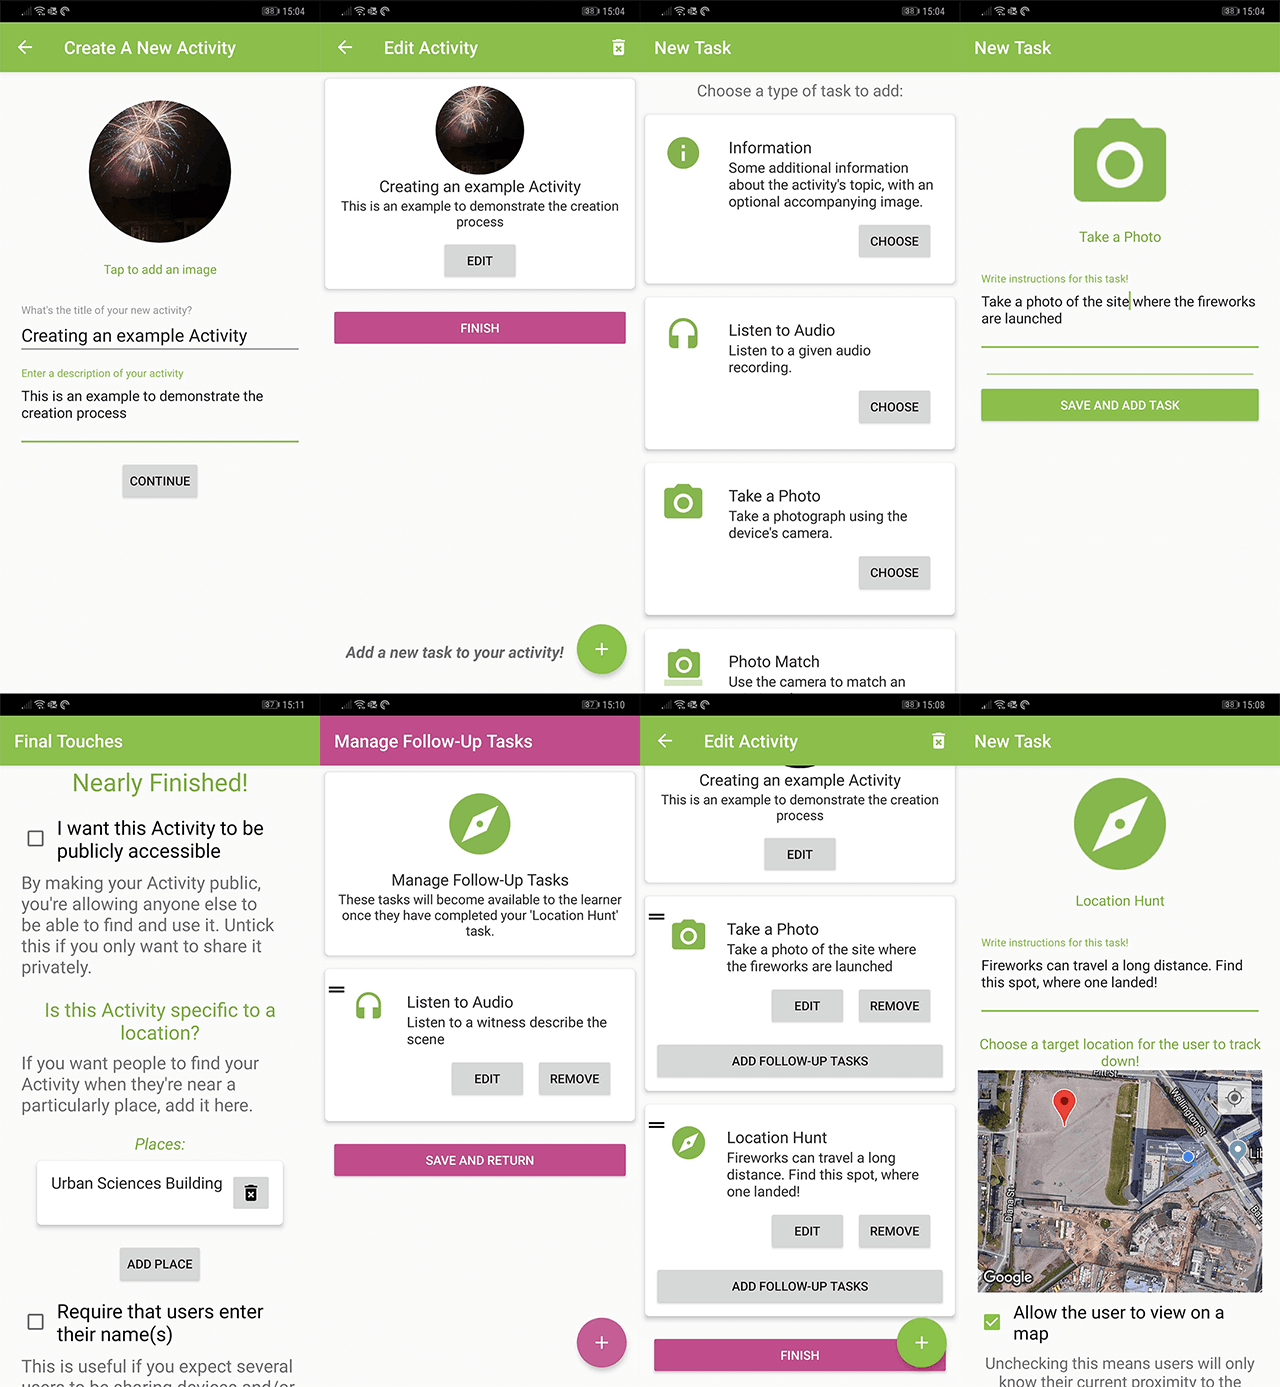
\includegraphics[width=1\columnwidth]{images/chapter05/creation.png}
  \caption[Creating an OurPlace activity]{Creating an OurPlace activity (clockwise, from top left): a) Choosing the activity's title, description and image; b) The Activity overview screen; c) Choosing a Task Type to add; d) Adding a basic \textit{Take a Photo} Task, with a description, e) Adding a more complicated \textit{Location Hunt} Task, with description and target coordinates; f) The new Tasks in the Activity overview; g) Adding Follow-Up Tasks to the \textit{Location Hunt}; h) The final touches before uploading }~\label{fig:ActivityCreation}
\end{figure*}

Every Task Type requires some form of written instruction/information, but some also require or allow additional customization (addresses \hyperref[DG3]{DG3}). For example, the \textit{Take a Photo} Task Type only requires a written instruction for the learner to follow (e.g. "Take a photo of the site where the fireworks are launched" [Figure \ref{fig:ActivityCreation}.d]), while a \textit{Location Hunt} also requires the author to mark a location for the learner to find [Figure \ref{fig:ActivityCreation}.e]. Some Task Types require the author to supply some media, which can either be generated through the OurPlace app directly, or imported from another source as noted earlier. The media creation tools are the same as those used when `consuming' an Activity, again meaning that users who have previously completed an Activity have some understanding of the interface. For example, when creating a \textit{Listen to Audio} Task, the author must supply an audio recording: this can either be imported from an external source (as an MP3 file), or created using the same interface as the \textit{Record Audio} Task Type [Figure \ref{fig:TaskTypes2}.d]. If the author has made a mistake while creating a Task, such as a typo in its instructions, the contents can easily be edited and corrected.

Follow-Up Tasks can be added by simply tapping the `Add Follow-Up Tasks' button on any Task in the main list. This will open a new screen, where the author can add Follow-Up Tasks to a new list in the same manner as before [Figure \ref{fig:ActivityCreation}.g]. If a top-level Task has Follow-Up Tasks configured for it, the `Add Follow-Up Tasks' button changes to `Manage Follow-Up Tasks'.

Once happy with their Activity, the author presses `Finish' and is shown a `Final Touches' screen [Figure \ref{fig:ActivityCreation}.h]. Here they can configure some of the metadata attached to their Activity. They can choose whether their Activity should be publicly accessible or private, which will affect how others are able to access it (discussed in Section \ref{sec:SharingActivities}). Activities are set to public by default, to encourage a greater amount of content to be made accessible on the platform. Authors can also choose to associate the Activity with multiple locations (i.e. if the Activity is about that location). Places are selected through the Google Maps app and searching using the Google Places API. Finally, the author is given the option of requiring learners to enter their name before submitting responses to the Activity. This is particularly useful to allow teachers to differentiate between students' submissions when they share devices and/or OurPlace accounts (addresses \hyperref[DG6]{DG6}).

After the author applies these final touches and taps `Finish and Upload', the Activity is packaged up and added to the upload queue. Once uploaded, users can access their Activities from the ‘My Creations’ tab on the app's main screen. Here they can view their Activities' share codes (see below), delete them, edit them or open and experience the Activities as a learner. Whilst creating an Activity the author's progress is saved every time a change is made, reducing the chances of progress being lost. Authors can resume the creation of unfinished Activities, meaning that they can be more easily created across several sessions and/or locations (\hyperref[DG2]{DG2}, \hyperref[DG6]{DG6}). However, whilst editing an Activity changes are not cached offline, in order to avoid confusion related to having several versions at once. Instead, the author must make the changes and immediately upload the new Activity.

After an Activity marked `public' is uploaded, it must be approved by a `trusted user' (i.e. a researcher) before other users can see it as a public Activity (see Section \ref{sec:SharingActivities}). Until then, it is treated as if it is private. Activities created by administrators are automatically approved and are immediately made public.

\subsection{Activity Collections}
Late into the project, the ability to create Collections was added in response to users' feedback. As their name implies, Collections are simply selections of existing Activities which share a commonality. They were added to the app for creations such as trails, where users wanted to have a full Activity's features at each stop, rather than being limited to a \textit{Location Hunt} and Follow-Up Tasks. Having opened a Collection, learners can optionally do a \textit{Location Hunt} to any Activities which have a location associated with them. At the time of writing, only the Android version of OurPlace supports Collections. After the introduction of Collections, the `My Activities' tab was renamed to `My Creations'.

\begin{figure*}
  \centering
  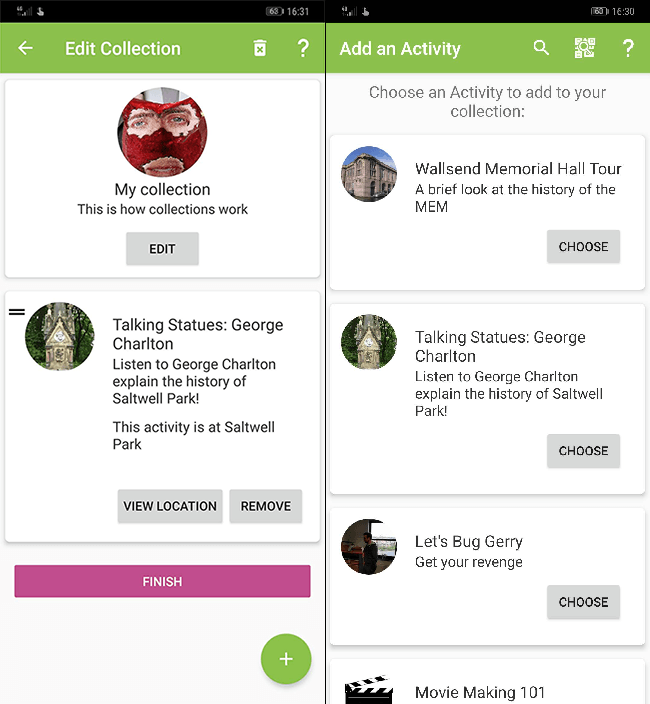
\includegraphics[width=0.5\columnwidth]{images/chapter05/CreateCollection.png}
  \caption[Creating an OurPlace Activity Collection]{Creating an OurPlace Activity Collection. Left to Right: A) The Collection creation screen looks very similar to the interface for Activity creation, with Activities listed instead of Tasks. B) The author's created Activities are listed for easy access, but they can also add other users' Activities by entering a Share Code or scanning a QR Code. }~\label{fig:CollectionCreation}
\end{figure*}

Collections are created in a very similar manner to Activities, with some of the screens being identical. A creator can give their Collections a title, description and optional image. Rather than adding Tasks, they add Activities [Figure \ref{fig:CollectionCreation}.A]. When adding an Activity to the Collection, the user is presented with their previously uploaded Activities for easy access [Figure \ref{fig:CollectionCreation}.B]. Should they want to create a Collection which includes other users' created Activities, they can select them either by entering the Activity's Share Code or scanning its QR Code (detailed in Section \ref{sec:SharingActivities}). Once finished adding Activities, users then note whether the Collection should be publicly accessible and what locations the Collection should be associated with (the list of places is auto-populated with the selected Activities' associated locations). As Collections are associated with Activities rather than copying/containing them, if an Activity held by a Collection is edited and updated, the Collection will reflect those changes. Collections go through the same approval process as Activities.

\subsection{Sharing, Discovering and Launching Creations}
\label{sec:SharingActivities}

In order to promote the use of the OurPlace app in authentic learning contexts (\hyperref[DG1]{DG1}, \hyperref[DG5]{DG5}, \hyperref[DG6]{DG6}) whilst also being adaptable to the various requirements of teachers, learners and place stakeholders (\hyperref[DG2]{DG2}, \hyperref[DG3]{DG3}, \hyperref[DG6]{DG6}), there needed to be a variety of options for content discovery and consumption. Key to our response to this issue was the choice to have the Creation author be in control of whether an Creation is public or private. Once approved by a trusted user, public Creations become visible in other users' Highlights Feed, while authors of private Creations have much more control over who can see them. 

\subsubsection{The Highlights Feed and Location}
Approved public Creations can appear in other users' Highlights Feed. As this tab is shown to all users upon opening the application, it means that many users will potentially see anything posted onto it. There are two ways that Creations can appear on the Highlights Feed: either by being one of the most recently uploaded pieces of content (and shown in a `Recently Uploaded' section of the feed), or being associated with a location which the user is close to. If the user has granted OurPlace permission to access their location, the server will return any and all places within 2.5km of the user which have Creations associated with them. These Creations are then listed in separate sections of the Highlights Feed, with one section for each location. This way, the system will always provide the user with some content, but prioritises Creations which have been made nearby (\hyperref[DG1]{DG1}, \hyperref[DG5]{DG5}) without the need for any additional user input (\hyperref[DG4]{DG4}).

\subsubsection{Share Codes and QR Codes}
All Creations, both public and private, have unique six character `share codes' associated with them. Authors can see the code for a Creation by tapping it in the `My Creations' tab, or by going onto the `Your Activities' section of the OurPlace website. Authors can then share this code with other users. The code can be entered (case insensitive, for ease of use) into the app's search function, which will immediately launch the Creation. Once opened, the Creation is cached so that the code doesn't have to be entered again to re-open it. 

QR Codes are also generated for each uploaded Creation, and made available to authors on the OurPlace website. The OurPlace app includes a simple QR code scanner, which will immediately launch a recognised Creation upon a successful scan. If the QR code is scanned on a device outside of the OurPlace app, the device's operating system will suggest that OurPlace be used to open the QR code if it is installed. If the app isn't installed, the user is taken to a web page with some information about the scanned Creation, and instructions for installing the OurPlace app to open it.

As these are the only methods of finding and launching private Creations, authors can have much greater control of who can access their creations, as well as where and when they do so (\hyperref[DG3]{DG3}). For example, a teacher can show Creations' share/QR codes on their classroom projector, so that students can easily download particular Creations prior to a school trip (\hyperref[DG2]{DG2}). Place stakeholders could also ensure that a Creation could only be accessed at a particular location by making it private, and featuring a QR code on an interpretation board (\hyperref[DG5]{DG5}). 

\section{The OurPlace Website}
\label{sec:ImplementationWeb}
In order for the OurPlace application to support the uploading and downloading of user Creations, responses and media, a remote web component was required. OurPlace's online server features both a website (for user-facing interactions) and an API (for the app's networking features). These are hosted within the European Economic Area on Microsoft's Azure Cloud infrastructure, using Azure's App Service and Storage systems for computation, networking and blob (file) storage.

The OurPlace website exists primarily as a management tool for the user's OurPlace content. Users can log into the website using the same account as they use for the mobile application, and are able to view their uploaded Activities (at the time of writing, Collections are not yet shown on the website) and responses, as well as responses to their created Activities (access given with the learner's consent). Activities cannot be created or opened through the website, although this functionality has been frequently requested. 

\begin{figure*}
  \centering
  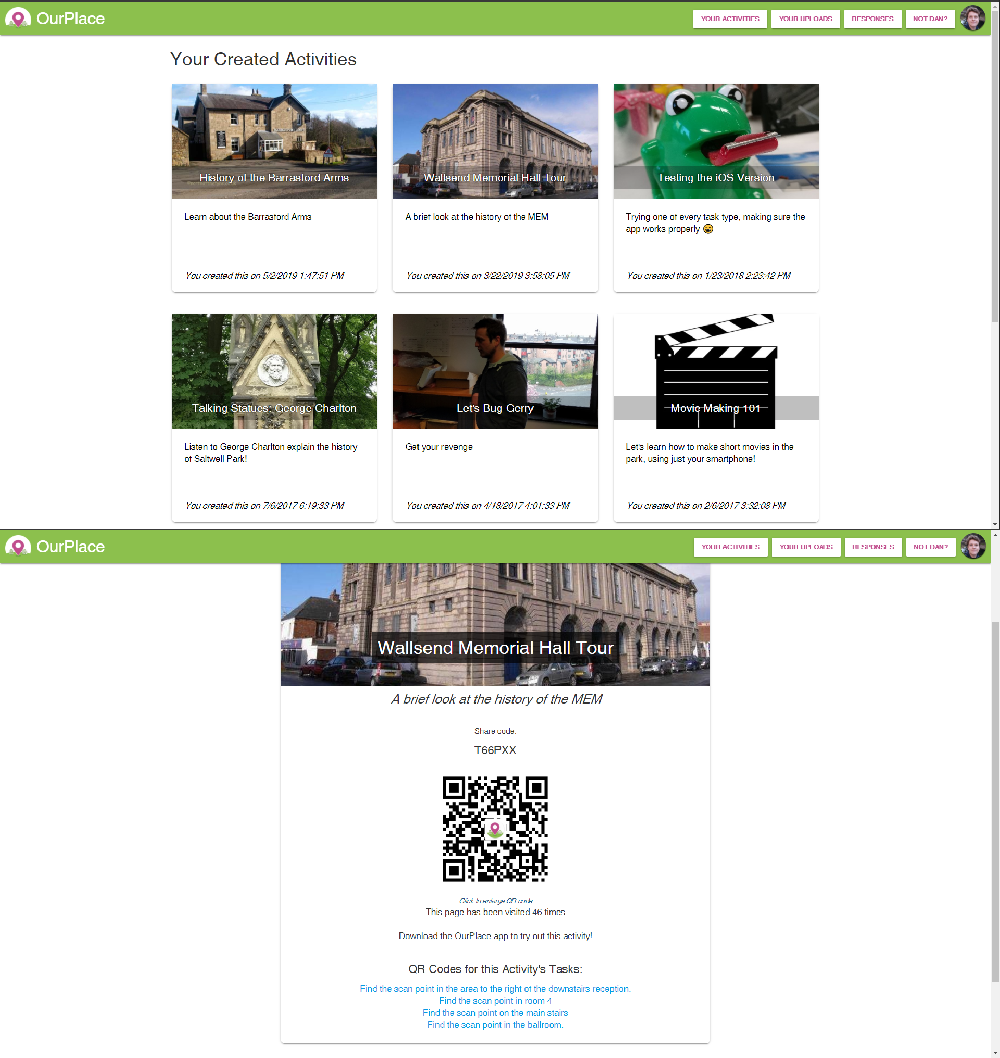
\includegraphics[width=0.85\columnwidth]{images/chapter05/webActivities.png}
  \caption[The OurPlace website: the user's Activities]{Viewing the user's created Activities on the OurPlace website. Top: the user can see all of their uploaded Activities on the website. Bottom: When an Activity is clicked, the user is shown some extra details, including its share code and QR code, as well as links to any QR codes needed for `Scan the QR Code' Tasks.}~\label{fig:websiteActivities}
\end{figure*}

Instead, the website is designed to be used for reviewing existing content. The `Your Activities' page will list all of the user's uploaded Activities [Figure \ref{fig:websiteActivities}]. When one is clicked, the user can see the Activity's QR and share codes, how many times that page has been accessed (i.e. how many times that QR code has been scanned), and access any QR codes needed to be printed for `Scan the QR Code' Tasks. The `Your Uploads' lists all of the user's uploaded responses to Activities [Figure \ref{fig:websiteResults}]. If an Activity requires that the learner enter their name before submission, the name will be displayed on the submission's card on this page (useful for when different people will be using the same device/account, addressing \hyperref[DG6]{DG6}). When a submission is clicked, the user is taken to a page where they can view the submission in its entirety. This page shows each Task in the Activity, in a format extremely similar to that found in the mobile app (\hyperref[DG4]{DG4}). The page's large elements are designed to be suitable for use on large displays, with the intention of supporting viewing submissions on devices such as classroom projectors (\hyperref[DG2]{DG2}). All submitted text, audio, video, images and map data can be viewed, and the user can enlarge the visual media for a closer look.

\begin{figure*}
  \centering
  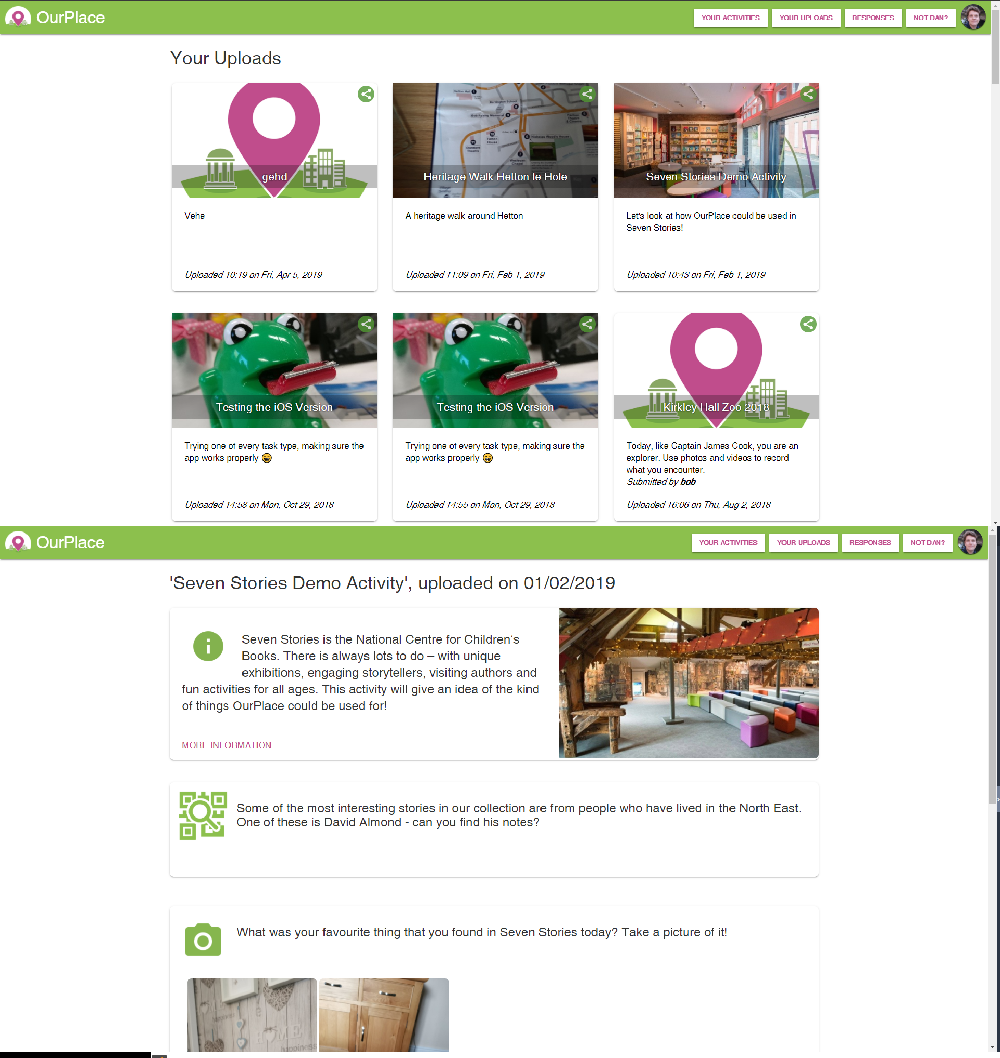
\includegraphics[width=0.85\columnwidth]{images/chapter05/webResults.png}
  \caption[The OurPlace website: the user's responses]{Viewing the user's uploaded responses on the OurPlace website. Top: the user can see all of their uploaded responses to Activities. Bottom: When a response is clicked, the user is shown its contents, in a format similar to the OurPlace mobile app.}~\label{fig:websiteResults}
\end{figure*}

A version of this page can also be accessed through the URL supplied by the `share' icon found on each card on the `Your Uploads' page. When followed, this `magic link' will allow anyone to view the submission without needing to be signed into an account---useful for sharing uploaded results with external collaborators, without sharing account access (\hyperref[DG3]{DG3}).

The `Responses' page is functionally very similar to the `Your Uploads' page, but lets the user see what other learners have submitted in response to Activities that the user has created. These responses are only made available to the user with the learner's explicit consent, given prior to uploading in the OurPlace app.

\section{Overview of the Technology}
The OurPlace platform is not insignificant, consisting of a smartphone application, a website and an online application programming interface (API). It was decided that in order to support as many schools, groups and individuals as possible, both of the main smartphone/tablet operating systems should be supported (Android and iOS). As a result, some consideration had to be made as to how the platform should be implemented on a technical level. This section covers the more technical decisions that had to be made, and a brief overview of the project's technical implementation.

\subsection{Use of the Xamarin Framework}
While many cross-platform mobile applications rely on implementations such as websites or `write once, deploy anywhere' technologies, these frequently carried with them functional limitations, performance issues or unpolished user experiences. I wanted the application to provide a high quality experience which conformed to each mobile platform's expected design metaphors, supported access to all of the devices' hardware features and didn't require a constant internet connection, which these options didn't support (at the time). Previously, the solution would be to develop completely `native' applications, resulting in having to produce software in multiple programming languages: for example, Android applications are usually written in either Java or Kotlin, whereas iPhone apps are written in Objective-C. As I was the only developer on the project, dedicating large amounts of time to learning, developing, iterating and maintaining systems across multiple languages was unrealistic. 

In the end, the decision was made to develop the mobile applications using the Xamarin Framework. This framework takes code written in C\# and compiles it into `native' applications, meaning that apps look, feel and act like software written in the different platforms' specific languages. This gave the advantage of sharing the same programming language across both applications, without losing out on any major features and allowing for common code (functionality identical across the two applications, e.g. making requests to the server) to be shared across the projects. To fully capitalise on this code sharing advantage, it was decided to take this further and produce the website and API in C\#. As a result, every component of the OurPlace platform can be opened within the same Visual Studio `solution', significantly speeding up the development process.

While developing the mobile applications with the Xamarin framework significantly reduced to upfront time investment in the development process, it had trade-offs which became more apparent as the project grew. Having all of the OurPlace code available within one solution (discussed in \ref{sec:OurPlaceSolution}) was certainly convenient and minimised code duplication, but when combined with Xamarin's more demanding build process it created large performance overheads. This, combined with issues of documentation being in other programming languages (particularly on the iOS application), impeded the development workflow, frequently slowing it to a crawl. At the end of the project, it is difficult to say if significant time was saved by using Xamarin over the two platforms' `native' development tools. However, anyone considering these options should note that recent developments to Visual Studio and the Xamarin framework have significantly improved performance, which may somewhat mitigate these issues.

\subsection{The OurPlace Visual Studio Solution}
\label{sec:OurPlaceSolution}
All of the OurPlace code is open source, and can be viewed at \url{https://github.com/GSDan/OurPlace}. Using C\# and Microsoft's .NET Framework across the OurPlace platform afforded it being accessible within a single Visual Studio solution, split into four smaller component projects: \textit{OurPlace.Common}, \textit{OurPlace.API}, \textit{OurPlace.Android} and \textit{OurPlace.iOS}.

\paragraph{OurPlace.Common}
This is a .NET Standard 2.0 project, which acts as a `library' of functions and serves the other projects within the solution, avoiding duplicating large swathes of code. It contains shared data models, interfaces and common core functionality, including managing the apps' local files, authenticating with the API, polling for the latest OurPlace activities and uploading new activities and responses. This is the only project which is referenced from elsewhere in the solution.

\paragraph{OurPlace.API}
This project uses version 4.6.1 of the .NET Framework, and contains an MVC ASP .NET website, a Web API 2 powered API and a Code First, Entity Framework database. User authentication for the API and website are handled through OWIN OAuth 2.0, supporting user account creation and login through both Google and Facebook. The server, database and file storage are hosted on Microsoft's Azure cloud platform, and deployed directly from within Visual Studio. All of the website's pages have been designed to work on a wide variety of device types, comfortably supporting phones, tablets, laptops and projectors.

\paragraph{OurPlace.Android}
This project contains all of the code specific to the Android application. Written in C\# using the Xamarin.Android framework, a `native' Android application is produced upon compilation, supporting devices running Android versions as old as 4.1 (Jelly Bean, 2012) and targeting the latest features found in version 8.1 (Oreo, 2017).

\paragraph{OurPlace.iOS}
This project contains all of the code specific to the iPhone/iPad application. Written in C\# using the Xamarin.iOS framework, a `native' iOS application is produced upon compilation. The application requires a minimum of iOS 10, which is supported by devices as old as the iPhone 5 (released 2012).

\section{Summary}
In order to create a mobile learning application which could be utilised by both schools and communities for authentic, place-based civic learning, we created six design goals based off of existing literature and our preliminary findings. These were that the technology should: utilize local places and communities as learning resources; support seamless outdoor and classroom use; support a variety of pedagogical approaches and stakeholder requirements; support a wide range of user ages and technical expertise; support learning and reflection in authentic learning contexts; and support mobile learning in resource-limited schools.

In response to these design goals, we iterated upon the ParkLearn prototype, eventually creating the OurPlace app. While the original ParkLearn technology probe only supported users in consuming and responding to hard-coded learning material, the new application supported the creation of new mobile learning activities without the need for additional tools. These `Activities' are made up of smaller, modular interactions called `Tasks'. Each Task asks to user to perform an interaction, based on its `Task Type' (listed in Section \ref{sec:TaskTypes}). Many of these carry over from the ParkLearn prototype, and use interactions which either promote learner creativity or emulate previously existing learning material. Furthermore, responses to these Activities could be uploaded and viewed on the accompanying OurPlace website, designed for use in classroom activities. 

The OurPlace platform responded to the design goals by promoting strong ties to location-based interactions and content; supporting learning activities seamlessly across physical and social contexts, through the use of mobile devices and a desktop website; supporting various pedagogical and stakeholder requirements by offering a wide variety of potential combinations of interactions and deployment opportunities, while giving users control over who can access their creations; offering a visually simple, consistent interface and user experience; enabling deep reflection and engagement with local knowledge by supporting in-depth responses to (and the creation of) learning material in-situ; and providing measures which support device sharing and offline storage of Activities and responses.